\documentclass[10pt]{article}
\usepackage[letterpaper,top=0.75in,bottom=0.75in,left=0.75in,right=0.75in]{geometry}
%\usepackage{geometry}
\usepackage{graphicx}
\usepackage{amssymb}
\usepackage{amsmath}
\usepackage{enumerate}
\usepackage{float}
\setlength\parindent{0pt}

\title{
\vspace{-20.mm}
Privacy Preserving Biometrics based Remote Authentication Protocol for Mobile Devices}
%\date{}
\date{\vspace{-5ex}}
%\vspace{-20.mm}

\begin{document}
\maketitle
Faculty supervising the research: Professor Elisa Bertino.\\
PhD student nominated:\quad \quad \quad \quad Hasini Gunasinghe.
\section{Motivation}
There has been a major shift from traditional passwords based authentication to biometrics based authentication in consumer applications in the 
recent past as major service providers such as the leaders in banking~\cite{citi, hsbc, usaa}, credit cards~\cite{mastercard} and 
e-commerce~\cite{amazon, alibaba} are adopting biometrics to authenticate users.
Biometrics is a strong authentication factor due to its ability to uniquely identify an individual. Different 
vendors have adopted it for different motivations. For example, Amazon uses selfies based on facial recognition techniques to avoid the difficulty of typing passwords to authenticate transactions in mobile devices with small screens~\cite{amazon}; Master Card has adopted it in order to 
drastically cut-down the cost of falsely declined transactions~\cite{mastercard}.

Two main contexts in which biometrics is being used for authentication are: in-person authentication~\cite{google} and remote 
authentication~\cite{hsbc}. In the first case, the user is present at the authenticator's premise when authentication is performed 
%and a device of the autheticator captures the biometrics. 
whereas in the second case, authentication is performed over the network. 
%and the biometrics is captured by the user's device. 
While there are common challenges w.r.t both cases due to sensitivity as biometrics is tightly coupled with one's identity, non-repeatability as no 
two biometrics samples of the same individual match exactly, and non-revocability as biometrics cannot be canceled/revoked, the second case is more 
challenging than the first one due to spoofing attacks, attacks on the communication channel, and attacks on the user's device. 
%Furthermore, remote biometrics based authentication is being widely 
%used since online-banking and e-commerce applications are increasingly adopting it.

%COMMENT: the discussion is not very good from a logical point of view. In
%the above paragraph you talk about the network attacks; in this paragraph you talk about
%attacks on the databases storing templates; then again you talk about insecurity
%arising from the transmission of raw template. So it seems that you keep repeating 
%overlapping problems in different places. Can you re-organize the discussion?
Remote commercial authentication systems being deployed today have key security problems irrespective of whether they incorporate state-of-the-art facial/voice recognition algorithms and liveliness verification techniques. 
First, since users' biometrics templates are stored in the server databases for matching during the authentication, these databases become major targets 
of attackers.
For example, in Google Hands Free system~\cite{google}, user's picture taken at the authentication time is matched with the user's Hands Free 
profile picture. In the Citi bank system, the user's pre-recorded voice samples are matched with the voice captured when the user call in. Second, 
multiple third party service providers store different biometrics traits of the same user (such as face, voice and fingerprint) for their 
proprietary authentication protocols. This creates multiple points of vulnerability on one's biometrics identity, due to 
linkability~\cite{linkability}. Third, the current protocols require the users to send a raw biometrics sample over the network each time the user 
remotely authenticates using biometrics, which is not desirable. 
Stolen biometrics templates lead to identity theft which poses severe threat to user's 
digital identity, compared to the case in which a password is stolen, because biometrics samples reveal sensitive features of the user's 
biometrics identity which can not be revoked.
%non-revocable nature of the biometrics.

Therefore, it is critical that secure biometrics 
based remote authentication protocol to not require storing and transmitting sensitive biometrics information during authentication.
%because we can not solely rely on 
%encryption to protect biometrics databases and authentication channels as there have been many instances of 
%password breaches in the past, although such techniques were used to secure passwords during storage and transmission.
The second issue mentioned above can be addressed by introducing a trusted identity provider (IDP) to enroll user's biometrics identity~\cite{google, 
identityX}. However, if the IDP is involved in each transaction in which the user authenticates, such approach undermines the user's privacy since the IDP learns information 
about different transactions that the user performs with different service providers (SPs).
  
To address aforementioned security and privacy issues, we aim to develop a biometrics based remote authentication protocol which addresses the 
following requirements:
\begin{enumerate}
 \item The user's biometrics identity is enrolled with only a trusted IDP (i.e: biometrics is not stored with multiple SPs).
 \item The sensitive features of user's biometrics are not stored anywhere.
 \item The sensitive features of user's biometrics are not revealed during authentication.
 \item After the initial enrollment with the IDP, users can carry out biometrics based authentication with multiple SPs without 
involving the IDP. (i.e: user-centric as opposed to traditional IDP-centric authentication protocol).
 \item Enrolled biometrics identity is revocable and renewable.
 \item Efficiency in terms of computation and communication in order for it to be carried out from user's mobile devices.
\end{enumerate}

In what follows we describe our roadmap for designing and developing a privacy preserving biometrics based remote authentication protocol which addresses the above requirements.

\section{Past and on-going research work}
In our past research we have determined that zero knowlede proof (ZKP) of identity~\cite{fiat-shamir} is a suitable cryptographic primitive to be used along with a secure commitment 
scheme~\cite{pedersenCommitment}, in order to perform biometric-based authentication with a SP without revealing any sensitive biometrics information to the SP . The concept of ZKP of 
identity, first proposed by Feige, Fiat and Shamir~\cite{fiat-shamir} in 1988, has been used to develop numerous identity based authentication 
schemes~\cite{idemixConcepts, DAA} for static identities such as email, credit card number, etc. Making it applicable to the domain of biometrics 
based remote authentication is not straightforward due to non-repeatable nature of biometrics identity. 
%omit following sentence if needed%
Since the biometrics sample used to create the commitment does not exactly match the biometrics sample captured during 
authentication, the ZKP might not succeed even for the genuine prover, unlike in the case of static identity.
Previous approaches which addressed the non-repeatability issue of biometrics, mainly in the domain of biometrics based encryption, have used 
distance matching with threshold, by applying error correction techniques to the features extracted from the second sample. 
Our goal is to generate a unique, repeatable and revocable biometrics based identifier for the user, to be used in creating the identity 
commitment during the enrollment of identity and to be used in authentication via ZKP of identity. We employ a machine 
learning based classification model to generate such biometrics identifier (BID), based on the discriminative features of the user's biometrics.

\subsubsection*{Overview of the solution}

In what follows we provide an overview of the protocol that we have proposed, using the aforementioned building blocks. Please refer to our 
paper~\cite{ours} for more details. This protocol involves three main parties namely: IDP, SP, and user. It involves two main phases namely: 
enrollment phase and authentication phase.\\

\textbf{Enrollment Phase:}
First, the IDP trains a classification model using the biometrics features extracted from biometrics images. The output is a 
file encapsulating the base-classification model that encodes the information required for prediction. 
During enrollment of each user, the base classification model is customized by randomizing the class labels encoded in the 
model. This step is performed as a security measure to protect the BIDs of the other users of the system, if one user's device is compromised.
Features extracted from the biometrics image of the enrolling user are given as input to the customized classification model and the corresponding 
class label is obtained through prediction. This class label is combined with the user provided secret to generate the BID, which is used in creating 
the identity commitment. The identity commitment, which is based on the Pedersen commitment scheme~\cite{pedersenCommitment}, takes the form: $C (x, 
r)$ = $g^{x}h^{r} mod p$, where $x$ = BID and $r$ = user provided secret. Password based key generation is used to derive multiple secrets used in 
the protocol from a single password provided by the user. The BID generated according to our strategy preserves its uniqueness as it is based on the 
discriminatory features of the user's biometrics, is repeatable based on the prediction accuracy of the classification model, and is revocable as the 
user can cancel any existing BID and obtain a new one simply by requesting the IDP to issue a new customized classification model, which will return 
a different class label, and by changing the password from which the secret used to create the BID is derived.
At the end of the enrollment process, the user is issued an identity token (IDT) which contains the identity commitment signed by the IDP and the 
customized classification model, to be used during the authentication phase, which are securely stored in the user's device.\\

\textbf{Authentication Phase:}
During the authentication phase, the user provides the IDT issued by the trusted IDP, to the SP and carries out a ZKP of the biometrics identity with 
the SP.
The authentication succeeds if the user is able to prove the SP in zero-knowledge, his/her ownership of the biometrics identity and the knowledge of 
the secret encoded in the identity commitment recorded in the IDT. In order to carry out the proof, features extracted from a new biometrics image of the user 
are given as input to the customized classification model stored in the user's device and the BID is generated according to the same steps used for the BID generation in the 
enrollment phase. This BID and the secret derived from the user's password are used to carry out the ZKP of biometric identity.\\

Our protocol~\cite{ours} complies with the first five requirements mentioned in Section 1. The research goal of the current  semester (Spring 2016) is to implement it in the mobile device and to evaluate the performance in order to assess its efficiency.

\section{Next research goal}
In our solution, we assume the support of a Trusted Execution Environment  (TEE) in the user's mobile device to securely store the 
artifacts obtained from the IDP during the enrollment phase and to execute the BID generation process using the classification model during the 
authentication phase. 
TEE isolates the storage and the execution from other applications that run in the device which provides protection against Trojan type attacks, in 
addition to just providing encrypted storage for the artifacts. TEE is used by Apple touch ID and Android fingerprint authentication framework as well.
Although there are extensive research on the develpment of TEE technology~\cite{tee}, there are attacks that have been discovered~\cite{blackhat} on 
them too.
Since widely used implementations of TEE technology such as ARM's TrustZone are proprietary and are not disclosed for public review, the level of 
assurance provided against a given threat model is unclear~\cite{armtrustzone}. 

Furthermore, recent advances in memory forensics techniques~\cite{dimsum} have introduced new privacy threats as these techniques show is that is 
possible to recover data from memory images even long after the processing of the data has completed. 
Although it is theoretically possible to clear the related memory upon destruction of a process, such approach is not practical because it requires 
accurate tracking of each data object, which is a very heavy-weight operation that no commodity operating system performs.

Therefore, our next research goal is to develop a biometrics based authentication protocol which achieves all the security and 
privacy goals mentioned in Section 1, based only on theoretical foundations and without assuming any platform security support. Fully homomorphic 
encryption (FHE)~\cite{fhe} is one solution that does not require decryption of sensitive information during authentication. However, FHE has several 
limitations, including: the SP learns the authentication function, which is the classification model 
in our case; and SP needs to obtain the secret key to decrypt the authentication decision, which in turn allows the SP to decrypt the biometrics data 
as well. 
Yao's garbled circuit~\cite{yaogc}, on the other hand, is a better cryptographic 
building block as it allows secure computation of a function $f$ on an input data $x$ to obtain the result $f(x)$ while hiding both the function and the 
input data from the function evaluator.\\

\textbf{Overview of the proposed solution}\\
In what follows we present the initial design of the solution that we aim to develop next.\\
\begin{figure}[h]
\centering
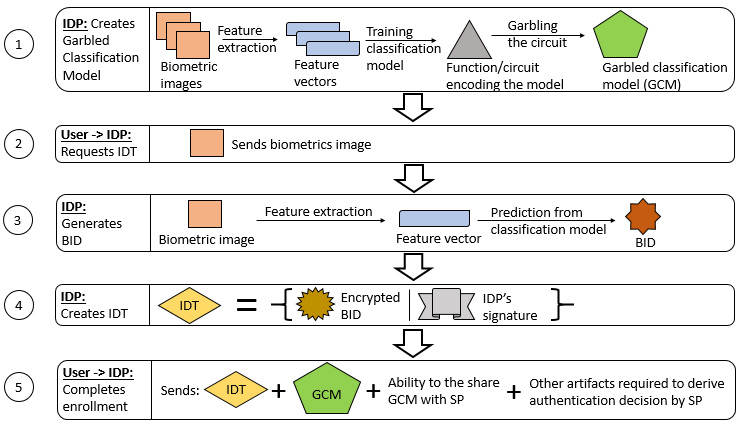
\includegraphics[height=3.00in,width=5.00in]{enrollment}
\caption{Proposed Enrollment Phase}
\label{example}
\end{figure}
\begin{figure}[h]
\centering
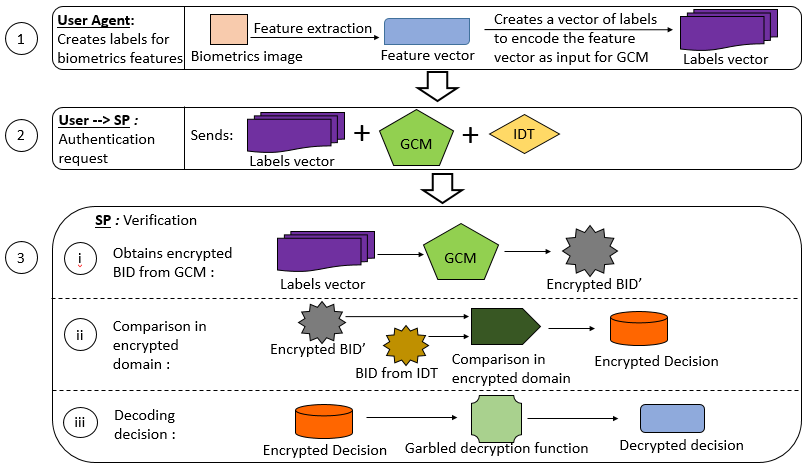
\includegraphics[height=3.00in,width=5.00in]{authentication}
\caption{Proposed Authentication Phase}
\label{example}
\end{figure}

\textbf{Enrollment Phase:}
As shown in Figure 1, the IDP first creates a trained classification model (which is a function that can be encoded as a circuit) and then creates a 
garbled version of it (step 1). This is shared with the enrolling user, to be used during authentication, along with other artifacts and the IDT 
(step 5). The IDT in this case is the encrypted and signed BID of the user (step 4). The encryption used here facilitates the comparison in 
encrypted domain without requiring any secret key to decrypt the comparison result. This is achieved by providing a garbled version of the 
decryption function to the evaluator (see step 3.ii of Figure 2). The BID is obtained as the classification output of the biometrics features of the 
user which is given as input to the trained classification model (step 2).\\

\textbf{Authentication Phase:}
The authentication phase is illustrated in Figure 2. Using the ability to share the GCM with the authenticator (i.e: SP) which is delegated by the IDP 
(step 5 of Figure 1), the user creates labels corresponding to the biometrics feature vector (step 1), for the SP to evaluate the GCM and obtain the 
encrypted BID (step 3.i).
During the verification, the SP compares in the encrypted domain, the output obtained in the step 3.i with the encrypted BID in the IDT issued by the 
IDP (step 3.ii). SP uses the provided garbled decryption function to obtain the decrypted authentication result (step 3.iii) without learning any 
other sensitive information about the user's biometrics.\\

\textbf{Challenges:}
One basic limitation of the original garbled circuit construction is that it offers only one-time usage. Specifically, evaluating a circuit on any 
new input requires an entirely new garbling of the circuit~\cite{reusablegc}. This requires the user to communicate with the IDP each time the user 
needs to authenticate to a SP, which we need to avoid as per the 4th requirement mentioned in Section 1. The problem of reusing garbled 
circuits has been open for 30 years until every recently when the notion of reusable garbled circuit construct was proposed by Shafi et. al in 2013~\cite{reusablegc}. This new 
construct sounds promising for the development of our target biometrics based authentication protocol, as it makes it possible to use multiple times the secure authentication 
artifacts that are issued upon enrollment (step 5 of Figure 1) without exposing any sensitive information during the authentication  
process.

Utilizing this construct in designing and developing our target biometrics authentication protocol, however, requires addressing several challenges. 
First, the scheme proposed in~\cite{reusablegc} is used in the context of two party secure computation protocols. We need to extend it to the case of a three-party 
secure computation protocol to build our solution, specifically as we need to address the question of how the IDP (which is the circuit generator) 
delegates the ability to the user (step 5 of Figure 1) to issue labels  to the SP(s) (step 1 of Figure 2) for the SPs to evaluate the garbled 
classification model (step 3.1 of Figure 2). 
Second, encoding the classification model as a garbled function is a challenge. Very recent 
efforts~\cite{mlgc} have focused on developing building 
blocks to construct privacy preserving classifiers which will be useful in addressing this challenge.
Third, we need to investigate whether it is possible to combine the three substeps in the step 3 of the authentication phase into one garbled 
circuit or whether these substeps must be executed separately, based on technical feasibility, security and efficiency.
Fourth, we need to make sure that delegation of the ability to share the GCM by the IDP to the user does not require storing secret information at 
the user's device.
Fifth, all the existing efficient implementations of garbled circuits do not support this construct, which is a  major implementation challenge of our 
protocol.

Therefore, we believe that addressing such challenges and developing a design and implementation of a secure and privacy preserving biometrics 
authentication protocol using this construct will result in groundbreaking contributions to the area of remote, privacy-preserving, and strong 
authentication techniques, and may also contribute to enhance current products. Finally we believe that, as the proposed architecture is modular and 
independent from specific device hardware characteristics, that our protocols and software tools can be used also for authentication in IoT 
(Internet-of-Things) contexts and can be easily transferred as a commercial product.
\subsubsection*{Contribution of this work:}
We aim to produce the following research output:
\begin{enumerate}
 \item Designing a secure and privacy preserving biometrics based remote authentication protocol which complies with the requirements listed in section 1, using re-usable 
garbled circuit construct. 
 \item A prototype implementation of the protocol that is able to run in mobile devices.
 \item Security and performance analysis of the protocol.
\end{enumerate}
\footnotesize
\bibliographystyle{IEEEtran}
\bibliography{IEEEabrv,IEEEexample}
 
\end{document}
